\section{Casos de Uso Reales}
\begin{center}
\begin{figure}[H]
	\centering
	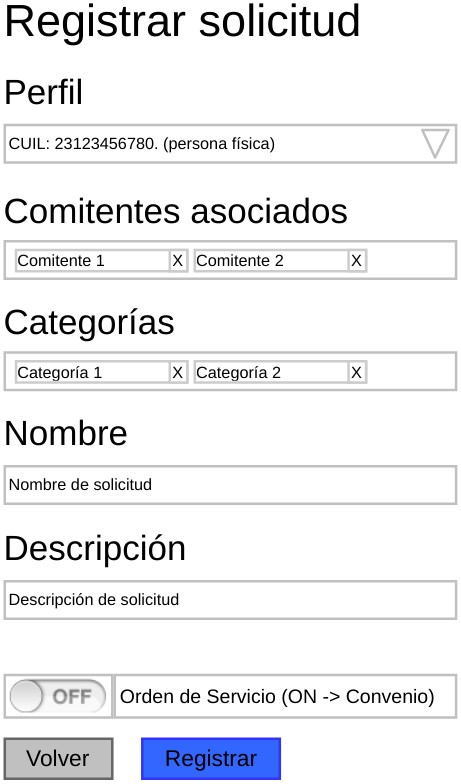
\includegraphics[width=0.5\linewidth]{registrarSolicitud}
	\caption{Interfaz de usuario para CUR-01}
\end{figure}
\hypertarget{CUR-01}{%
\begin{longtable}{ | p{3cm} | p{6.25cm} | p{6.25cm} | }
	\hline
	\rowcolor{lightgray}
	\hfil \textbf{\textit{CUR-01}} &
	\multicolumn{2}{ p{13cm} | }
		{\hfil \textbf{Registrar solicitud}} \\
	\hline
	\endhead
	\raggedleft \textit{Actores} & 
	\multicolumn{2}{ p{13cm} | }{Comitente} \\
	\hline
	\raggedleft \textit{Prop\'osito} &
	\multicolumn{2}{ p{13cm} | }
		{Registrar la solicitud de un servicio.} \\
	\hline
	\raggedleft \textit{Pre Condici\'on} & 
	\multicolumn{2}{ p{13cm} | }{(ninguna)} \\
	\hline
	\raggedleft \textit{Pos Condici\'on} & 
	\multicolumn{2}{ p{13cm} | }
		{Una solicitud de servicio ha sido agregada.} \\
	\hline
	\raggedleft \textit{Descripci\'on} &
	\multicolumn{2}{ p{13cm} | }{%
	Un Comitente quiere solicitar un servicio,
	por lo que debe dirigirse a la secci\'on de
	solicitudes; as\'i puede moverse al apartado
	para crear una solicitud nueva, donde se
	adjunta el nombre para la solicitud y una
	descripci\'on de la misma; junto con los
	Comitentes asociados y categor\'ias
	correspondientes a la solicitud.} \\
	\hline
	\newpage
	\multirow{2}{3cm}{%
		\raggedleft
		\textit{Flujo t\'ipico de Eventos}
	} &
	\hfil Acci\'on del Autor &
	\hfil Respuesta del Sistema \\
	\cline{2-3} &%
	\begin{enumerate}[wide, labelwidth=!, labelindent=0cm]
		\vspace{-0.25cm}
		\item El Comitente se dirige a la
		secci\'on de solicitudes de servicios
		\vspace{1cm}
		\addtocounter{enumi}{1}
		\item El Comitente se dirige a la
		la secci\'on para agregar una nueva
		solicitud
		\vspace{0.75cm}
		\addtocounter{enumi}{1}
		\item El Comitente coloca el nombre y
		categor\'ia de la solicitud, y confirma
		la informaci\'on dada
	\end{enumerate} &%
	\begin{enumerate}[wide, labelwidth=!, labelindent=0cm]
		\addtocounter{enumi}{1}
		\item El sistema devuelve el listado de
		solicitudes de servicios con la secci\'on
		para agregar una nueva solicitud
		\vspace{0.5cm}
		\addtocounter{enumi}{1}
		\item El sistema proporciona el formulario
		para generar una solicitud de servicio nueva
		\vspace{1cm}
		\addtocounter{enumi}{1}
		\item El sistema guarda la nueva solicitud
		de servicio dada y proporciona la confirmaci\'on
		de la operaci\'on exitosa
	\end{enumerate} \\
	\hline
	\raggedleft \textit{Curso Alternativo de Eventos} &
	\multicolumn{2}{ p{13cm} | }{%
		\vspace{-0.25cm}
		\parbox{13cm}{%
		Pasos 5 y 6: El Responsable T\'ecnico completa el
		formulario de forma inadecuada. El sistema
		indica el error cometido y permanece
		en el mismo lugar.
		\vspace{0.25cm}
		}} \\
	\hline
\end{longtable}}
\clearpage
\begin{figure}[H]
	\centering
	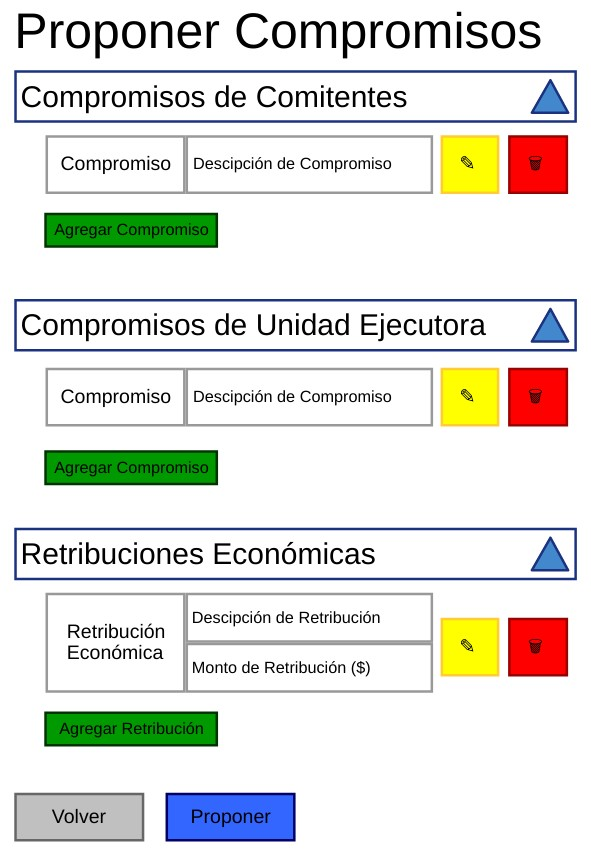
\includegraphics[width=0.5\linewidth]{proponerCompromisos}
	\caption{Interfaz de usuario para CUR-02}
\end{figure}
\hypertarget{CUR-02}{%
\begin{longtable}{ | p{3cm} | p{6.25cm} | p{6.25cm} | }
	\hline
	\rowcolor{lightgray}
	\hfil \textbf{\textit{CUR-02}} &
	\multicolumn{2}{ p{13cm} | }
		{\hfil \textbf{Proponer Compromisos}} \\
	\hline
	\endhead
	\raggedleft \textit{Actores} & 
	\multicolumn{2}{ p{13cm} | }{Responsable T\'ecnico} \\
	\hline
	\raggedleft \textit{Prop\'osito} &
	\multicolumn{2}{ p{13cm} | }
		{Gestionar las ABM de los Compromisos del Comitente,
		Compromisos de la Unidad Ejecutora y la Retribuci\'on
		Econ\'omica.} \\
	\hline
	\raggedleft \textit{Pre Condici\'on} & 
	\multicolumn{2}{ p{13cm} | }
		{Debe existir un ResponsableSolicitud que se vincule
		a esta solicitud, y tenga tiempo\_eleccion y
		tiempo\_adjudicacion no nulos.} \\
	\hline
	\raggedleft \textit{Pos Condici\'on} & 
	\multicolumn{2}{ p{13cm} | }
		{Los Compromisos del Comitente, los Compromisos
		de la Unidad Ejecutora y la Retribuci\'on
		Econ\'omica se han actualizado.} \\
	\hline
	\raggedleft \textit{Descripci\'on} &
	\multicolumn{2}{ p{13cm} | }{%
	Un Responsable T\'ecnico quiere adjuntar los recursos
	requeridos para un servicio solicitado, por lo que debe
	seleccionar la solicitud a la que tenga los permisos
	necesarios; entonces, agrega cada uno de los recursos
	(sea material, econ\'omico y/o humano) que se pretende
	involucrar.} \\
	\hline
	\pagebreak
	\multirow{2}{3cm}{%
		\raggedleft
		\textit{Flujo t\'ipico de Eventos}
	} &
	\hfil Acci\'on del Autor &
	\hfil Respuesta del Sistema \\
	\cline{2-3} &%
	\begin{enumerate}[wide, labelwidth=!, labelindent=0cm]
		\item El Responsable T\'ecnico selecciona
		la solicitud de servicio que se desea
		asignar recursos
		\addtocounter{enumi}{1}
		\item El Responsable T\'ecnico indica
		que quiere asignar los recursos para
		esta solicitud de servicio
		\addtocounter{enumi}{1}
		\item El Responsable T\'ecnico completa
		los Compromisos del Comitente y contin\'ua
		con el siguiente formulario
		\addtocounter{enumi}{1}
		\item El Responsable T\'ecnico completa
		los Compromisos de la Unidad Ejecutora y
		contin\'ua con el siguiente formulario
		\addtocounter{enumi}{1}
		\item El Responsable T\'ecnico completa
		la Retribuci\'on Econ\'omica y finaliza
		con la asignaci\'on de recursos
	\end{enumerate} &%
	\begin{enumerate}[wide, labelwidth=!, labelindent=0cm]
		\vspace{0.75cm}
		\addtocounter{enumi}{1}
		\item El sistema devuelve la solicitud
		del servicio indicada
		\vspace{0.25cm}
		\addtocounter{enumi}{1}
		\item El sistema proporciona el formulario
		para asignar los Compromisos del Comitente
		\addtocounter{enumi}{1}
		\item El sistema guarda los Compromisos del
		Comitente cargados y proporciona el formulario
		para asignar Compromisos de la Unidad Ejecutora
		\addtocounter{enumi}{1}
		\item El sistema guarda los Compromisos de
		la Unidad Ejecutora y proporciona el formulario
		para asignar la Retribuci\'on Econ\'omica
		\addtocounter{enumi}{1}
		\item El sistema guarda la Retribuci\'on
		Econ\'omica y comunica al usuario del \'exito
		de la operaci\'on
	\end{enumerate} \\
	\hline
	\raggedleft \textit{Curso Alternativo de Eventos} &
	\multicolumn{2}{ p{13cm} | }{%
		\vspace{-0.25cm}
		\parbox{13cm}{%
		Pasos 5, 7 y 9: El Responsable T\'ecnico
		completa el formulario de forma inadecuada.
		El sistema indica el error cometido y permanece
		en el mismo lugar.
		\vspace{0.25cm}
		}} \\
	\hline
\end{longtable}}
\clearpage
\begin{figure}[H]
	\centering
	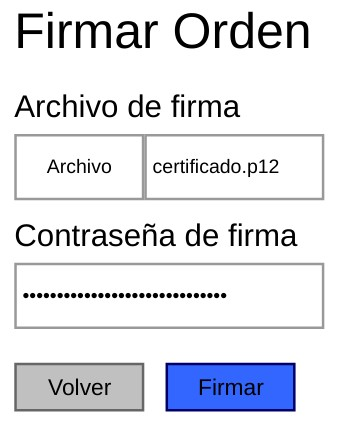
\includegraphics[width=0.3\linewidth]{firmarOrden}
	\caption{Interfaz de usuario para CUR-03}
\end{figure}
\hypertarget{CUR-03}{%
\begin{longtable}{ | p{3cm} | p{6.25cm} | p{6.25cm} | }
	\hline
	\rowcolor{lightgray}
	\hfil \textbf{\textit{CUR-03}} &
	\multicolumn{2}{ p{13cm} | }
		{\hfil \textbf{Firmar orden}} \\
	\hline
	\endhead
	\raggedleft \textit{Actores} & 
	\multicolumn{2}{ p{13cm} | }
		{Comitente, Responsable T\'ecnico y Secretario} \\
	\hline
	\raggedleft \textit{Prop\'osito} &
	\multicolumn{2}{ p{13cm} | }
		{Agregar una orden de servicio con una firma
		digital.} \\
	\hline
	\raggedleft \textit{Pre Condici\'on} & 
	\multicolumn{2}{ p{13cm} | }
		{El Comitente y los Responsables T\'ecnicos
		acordaron los Compromisos y Retribuciones
		para un servicio solicitado.} \\
	\hline
	\raggedleft \textit{Pos Condici\'on} & 
	\multicolumn{2}{ p{13cm} | }
		{Se registr\'o una nueva orden de servicio con
		una firma digital m\'as a la antecesora.} \\
	\hline
	\raggedleft \textit{Descripci\'on} &
	\multicolumn{2}{ p{13cm} | }{%
	Un actor decide firmar una orden de servicio digitalmente,
	por lo que debe dirigirse a la orden de servicio en
	cuesti\'on; entonces, coloca la firma en el documento
	y se agrega al conjunto de firmas que ya tenga.} \\
	\hline
	\newpage
	\multirow{2}{3cm}{%
		\raggedleft
		\textit{Flujo t\'ipico de Eventos}
	} &
	\hfil Acci\'on del Autor &
	\hfil Respuesta del Sistema \\
	\cline{2-3} &%
	\begin{enumerate}[wide, labelwidth=!, labelindent=0cm]
		\vspace{-0.75cm}
		\item El actor se dirige a la
		secci\'on de \'ordenes de servicios
		\vspace{1.5cm}
		\addtocounter{enumi}{1}
		\item El actor se dirige a la
		la secci\'on para firmar la orden
		de servicio
		\vspace{1cm}
		\addtocounter{enumi}{1}
		\item El actor carga la firma digital,
		junto con la contrase\~na de la misma,
		y confirma la informaci\'on dada
	\end{enumerate} &%
	\begin{enumerate}[wide, labelwidth=!, labelindent=0cm]
		\vspace{0.5cm}
		\addtocounter{enumi}{1}
		\item El sistema devuelve el listado de
		\'ordenes de servicios con la secci\'on
		para firmar la orden de servicio
		\vspace{0.5cm}
		\addtocounter{enumi}{1}
		\item El sistema proporciona el formulario
		para firmar digitalmente la orden de servicio
		\vspace{1.5cm}
		\addtocounter{enumi}{1}
		\item El sistema genera una nueva copia de la
		orden de servicio con la firma digital y
		proporciona la confirmaci\'on de la operaci\'on
		exitosa
	\end{enumerate} \\
	\hline
	\raggedleft \textit{Curso Alternativo de Eventos} &
	\multicolumn{2}{ p{13cm} | }{%
		\vspace{-0.25cm}
		\parbox{13cm}{%
		Paso 6: El archivo para firma digital proporcionado
		no corresponde a un certificado digital privado.
		El sistema indica el error cometido y permanece
		en el mismo lugar.
		\newline
		Paso 6: La contrase\~na proporcionada no descifra
		la firma digital proporcionada. El sistema indica
		el error cometido y permanece en el mismo lugar.
		\vspace{0.25cm}
		}} \\
	\hline
\end{longtable}}
\clearpage
\begin{figure}[H]
	\centering
	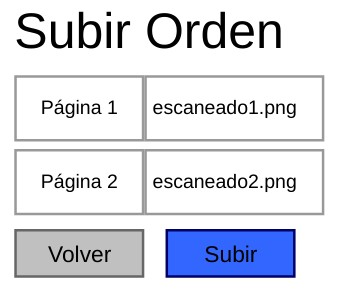
\includegraphics[width=0.3\linewidth]{subirOrden}
	\caption{Interfaz de usuario para CUR-04}
\end{figure}
\hypertarget{CUR-04}{%
\begin{longtable}{ | p{3cm} | p{6.25cm} | p{6.25cm} | }
	\hline
	\rowcolor{lightgray}
	\hfil \textbf{\textit{CUR-04}} &
	\multicolumn{2}{ p{13cm} | }
		{\hfil \textbf{Subir orden}} \\
	\hline
	\endhead
	\raggedleft \textit{Actores} & 
	\multicolumn{2}{ p{13cm} | }{Ayudante} \\
	\hline
	\raggedleft \textit{Prop\'osito} &
	\multicolumn{2}{ p{13cm} | }
		{Agregar una orden de servicio firmada de
		forma manuscrita, que fue escaneada.} \\
	\hline
	\raggedleft \textit{Pre Condici\'on} & 
	\multicolumn{2}{ p{13cm} | }
		{El Comitente, los Responsables T\'ecnicos y
		la Secretaria firmaron una orden de servicio
		impresa.} \\
	\hline
	\raggedleft \textit{Pos Condici\'on} & 
	\multicolumn{2}{ p{13cm} | }
		{Una orden de servicio firmada de forma
		manuscrita se encuentra en el sistema.} \\
	\hline
	\raggedleft \textit{Descripci\'on} &
	\multicolumn{2}{ p{13cm} | }{%
	Un Ayudante decide subir una orden de servicio impresa
	que se encuentra con todas las firmas requeridas,
	por lo que debe cargar el escaneo del papel en cuesti\'on;
	entonces, se verifica la validez del documento y
	se agrega al servicio que corresponda.} \\
	\hline
	\newpage
	\multirow{2}{3cm}{%
		\raggedleft
		\textit{Flujo t\'ipico de Eventos}
	} &
	\hfil Acci\'on del Autor &
	\hfil Respuesta del Sistema \\
	\cline{2-3} &%
	\begin{enumerate}[wide, labelwidth=!, labelindent=0cm]
		\item El Ayudante selecciona la opci\'on
		para subir una orden de servicio
		\addtocounter{enumi}{1}
		\item El Ayudante carga el escaneo de la
		orden de servicio y confirma la acci\'on
	\end{enumerate} &%
	\begin{enumerate}[wide, labelwidth=!, labelindent=0cm]
		\vspace{0.75cm}
		\addtocounter{enumi}{1}
		\item El sistema devuelve el formulario para
		subir una orden de servicio
		\addtocounter{enumi}{1}
		\item El sistema compara las similitudes entre
		la orden de servicio generada del sistema y
		lo escaneado
		\item El sistema comprueba que la orden de servicio
		escaneada posee los bloques de firma en el mismo
		lugar que la generada del sistema
		\item El sistema comprueba que hayan firmas
		dentro del documento escaneado
		\item El sistema comunica al usuario del \'exito
		de la operaci\'on
	\end{enumerate} \\
	\hline
	\raggedleft \textit{Curso Alternativo de Eventos} &
	\multicolumn{2}{ p{13cm} | }{%
		\vspace{-0.25cm}
		\parbox{13cm}{%
		Paso 4: El sistema no encuentra suficiente
		similitud entre la orden de servicio generada
		y el documento escaneado. El sistema indica la
		inconsistencia entre ambos. \\
		Paso 5: El sistema no encuentra los bloques
		de firma en el lugar esperado dentro del
		documento escaneado. El sistema indica la
		inconsistencia del archivo subido. \\
		Paso 6: El sistema no encuentra todas las
		firmas dentro del documento escaneado. El
		sistema indica la falta de reconocimiento
		de firmas.
		\vspace{0.25cm}
		}} \\
	\hline
\end{longtable}}
\end{center}
\section[Diagramas de Interacci\'on]
	{Diagramas de Secuencia de Dise\~no}
\begin{figure}[H]
	\centering
	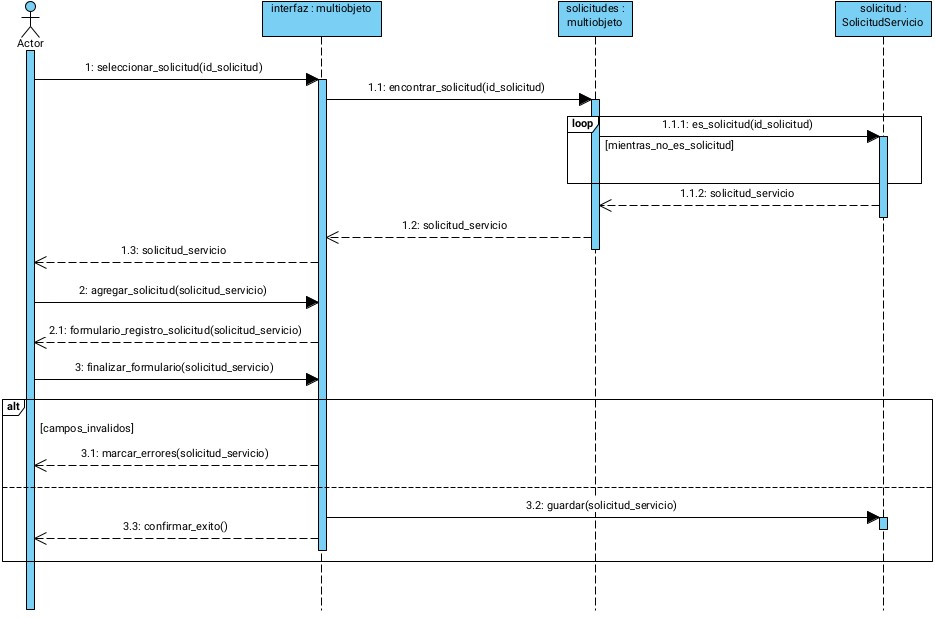
\includegraphics[width=\linewidth]{dsd1}
	\caption{DSD de CUR-01}
\end{figure}
\begin{figure}[H]
	\centering
	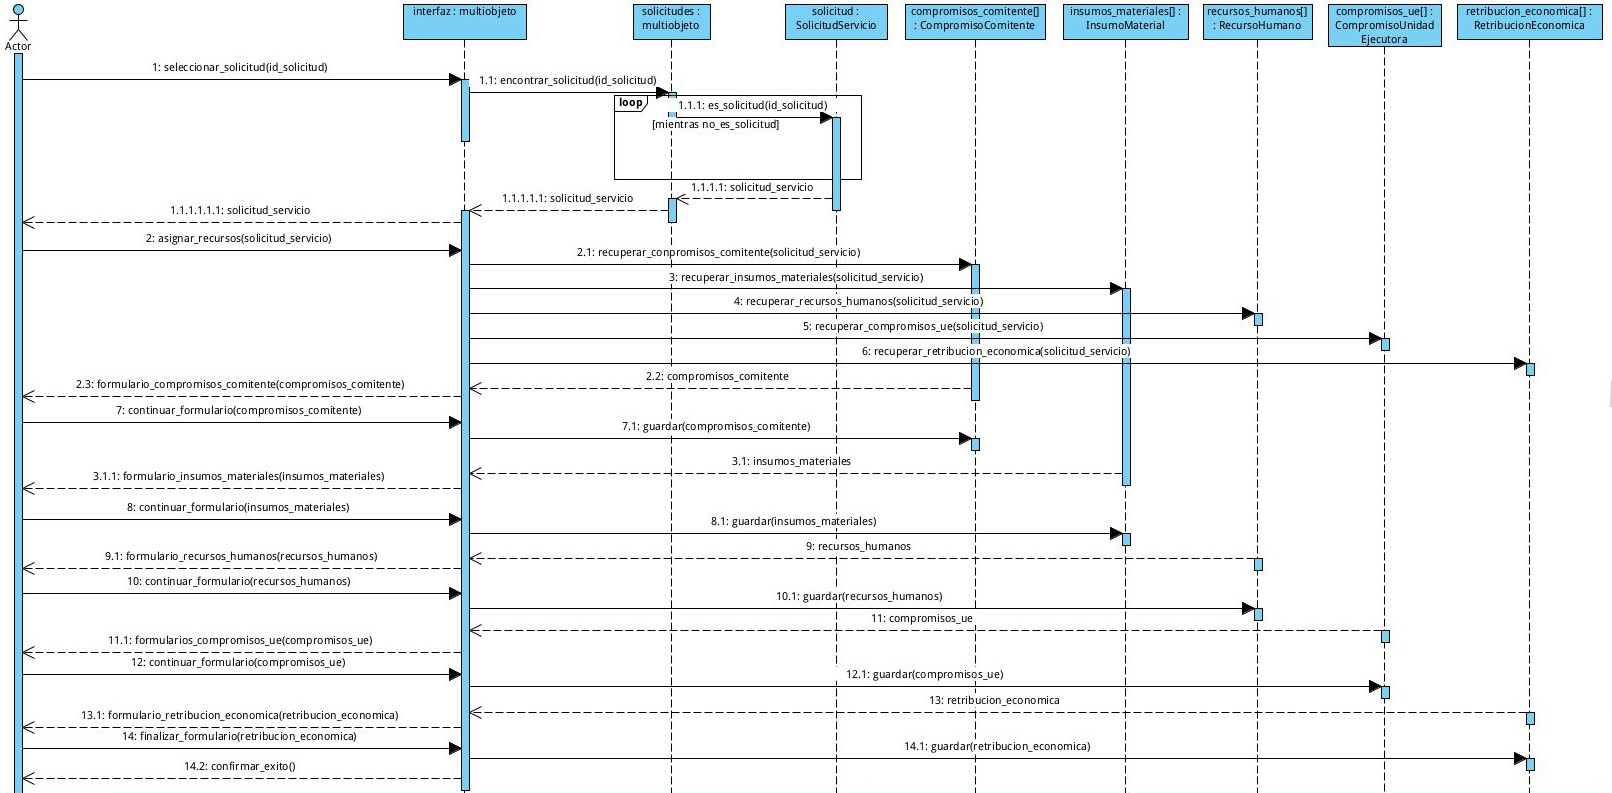
\includegraphics[width=\linewidth]{dsd2}
	\caption{DSD de CUR-02}
\end{figure}
\begin{figure}[H]
	\centering
	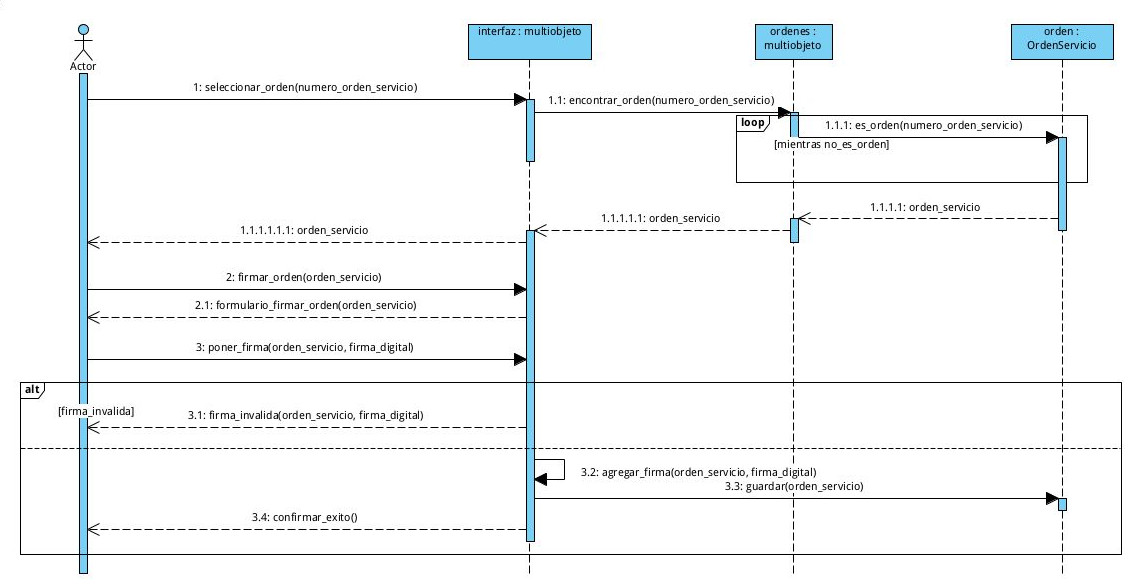
\includegraphics[width=\linewidth]{dsd3}
	\caption{DSD de CUR-03}
\end{figure}
\begin{figure}[H]
	\centering
	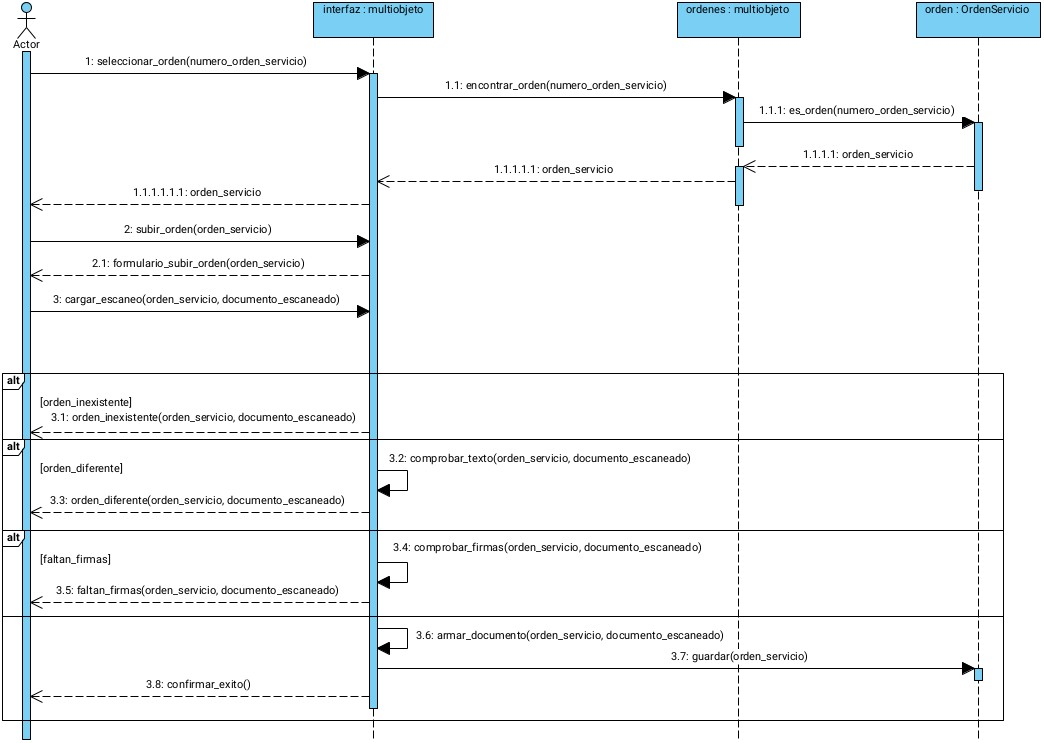
\includegraphics[width=\linewidth]{dsd4}
	\caption{DSD de CUR-04}
\end{figure}
\section{Diagramas de Clase}
\normalsize{\indent
Dado que en Python no hay elementos privados,
se prescinde de m\'etodos accesores y mutadores
de los atributos en todas las clases. Dentro
del diagrama, \textit{ts} significa timestamp.
}
\begin{figure}[H]
	\begin{center}
	\begin{tikzpicture}
		\umlclass[%
			text width=4.75cm,%
			x=-1, y=0%
		]{SolicitudServicio}{%
			nombre\_solicitud:str \\%
			descripcion\_solicitud:str \\%
			tiempo\_solicitud:ts \\%
			cancelacion\_solicitud:ts? \\%
			solicitud\_suspendida:bool%
		}{}
		\umlclass[%
			text width=7.5cm,%
			x=0, y=16%
		]{Comitente}{%
			cuil\_comitente:int \\%
			firma\_digital\_comitente:bool \\%
			habilitado\_comitente:bool \\%
			razones\_sociales\_comitente:str[] \\%
			cuit\_organizaciones\_comitente:int[] \\%
			puestos\_organizaciones\_comitente:str[] \\%
			habilitado\_organizaciones\_comitente:bool[]%
		}{}
		\umlclass[%
			text width=7cm,%
			x=0, y=8%
		]{ComitenteSolicitud}{%
			razon\_social\_comitente:str? \\%
			cuit\_organizacion\_comitente:int? \\%
			puesto\_organizacion\_comitente:str? \\%
			tiempo\_decision:ts? \\%
			aceptacion:bool%
		}{}
		\umlclass[%
			text width=8cm,%
			x=8.5, y=16%
		]{ResponsableTecnico}{%
			cuil\_responsable:int \\%
			firma\_digital\_responsable:bool \\%
			habilitado\_responsable:bool \\%
			razones\_sociales\_responsable:str[] \\%
			cuit\_organizaciones\_responsable:int[] \\%
			puestos\_organizaciones\_responsable:str[] \\%
			habilitado\_organizaciones\_responsable:bool[]%
		}{}
		\umlclass[%
			text width=7cm,%
			x=9, y=8%
		]{ResponsableSolicitud}{%
			razon\_social\_responsable:str? \\%
			cuit\_organizacion\_responsable:int? \\%
			puesto\_organizacion\_responsable:str? \\%
			tiempo\_decision\_responsable:ts? \\%
			aceptacion\_responsable:bool \\%
			tiempo\_decision\_comitente:ts? \\%
			aceptacion\_comitente:bool%
		}{}
		\umlclass[%
			text width=9cm,%
			x=8, y=-0.3%
		]{PropuestaCompromisos}{%
			descripciones\_compromisos\_comitente:str[] \\%
			descripciones\_compromisos\_unidad\_ejecutora:str[] \\%
			montos\_retribuciones\_economicas:Decimal[] \\%
			descripciones\_retribuciones\_economicas:str[]%
		}{}
		\umlassoc[%
			geometry=--, mult1=1, pos1=0.1,%
			mult2=0..*, pos2=0.75, align2= left,%
			anchors= -90 and 90%
		]{Comitente}{ComitenteSolicitud}
		\umlassoc[%
			geometry=--, mult1=1, pos1=0.2, align1= right,%
			mult2=1..*, pos2=0.95, align2= left,%
			anchors= 70 and -90%
		]{SolicitudServicio}{ComitenteSolicitud}
		\umlassoc[%
			geometry=-|-, mult1=1, pos1=0.3, align1= right,%
			mult2=0..*, pos2=2.3, align2= left,%
			anchors= 40 and 180%
		]{SolicitudServicio}{ResponsableSolicitud}
		\umlassoc[%
			geometry=--, mult1=1, pos1=0.2,%
			mult2=0..*, pos2=0.65, align2= left,%
			anchors= -81 and 90%
		]{ResponsableTecnico}{ResponsableSolicitud}
		\umlassoc[%
			geometry=--, mult1=1, pos1=0.15,%
			mult2=0..*, pos2=0.5, align2= left,%
			anchors= -15 and -175%
		]{SolicitudServicio}{PropuestaCompromisos}
	\end{tikzpicture}
	\end{center}
	\caption{Diagrama de Clases para Subsistema
	de Gesti\'on de Solicitudes}
\end{figure}
\begin{figure}[H]
	\begin{center}
	\begin{tikzpicture}
		\umlclass[%
			text width=4.75cm,%
			x=0, y=4%
		]{SolicitudServicio}{%
			nombre\_solicitud:str \\%
			descripcion\_solicitud:str \\%
			tiempo\_solicitud:ts \\%
			cancelacion\_solicitud:ts? \\%
			solicitud\_suspendida:bool%
		}{}
		\umlclass[%
			text width=4.75cm,%
			x=5.6, y=0%
		]{OrdenServicio}{%
			numero\_orden\_servicio:int \\%
			orden\_original:file? \\%
			orden\_firmada:file? \\%
			tiempo\_orden:ts \\%
			cancelacion\_orden:ts? \\%
			orden\_suspendida:bool%
		}{}
		\umlclass[%
			text width=5cm,%
			x=0, y=-2.5%
		]{Convenio}{%
			archivo\_convenio:file? \\%
			tiempo\_creacion\_convenio:ts \\%
			tiempo\_subida\_convenio:ts? \\%
			cancelacion\_convenio:ts? \\%
			convenio\_suspendido:bool%
		}{}
		\umlclass[%
			text width=5cm,%
			x=11.5, y=5%
		]{FirmaOrden}{%
			archivo\_firma\_orden:file? \\%
			tiempo\_firma\_orden:ts? \\%
		}{}
		\umlclass[%
			text width=6cm,%
			x=0, y=-9.5%
		]{Servicio}{%
			tiempo\_servicio:ts \\%
			cancelacion\_servicio:ts? \\%
			causa\_cancelacion\_servicio:str?%
		}{}
		\umlclass[%
			text width=5.5cm,%
			x=11, y=-5.5%
		]{Progreso}{%
			porcentaje\_progreso:Decimal \\%
			descripcion\_progreso:str%
		}{}
		\umlclass[%
			text width=5.5cm,%
			x=11, y=-9.6%
		]{Pago}{%
			monto\_pago\_servicio:Decimal \\%
		}{}
		\umlassoc[%
			geometry=-|, mult1=1, pos1=0.11,%
			mult2=0..1, pos2=1.5, align2= left,%
			anchors= 0 and 90%
		]{SolicitudServicio}{OrdenServicio}
		\umlassoc[%
			geometry=--, mult1=1, pos1=0.2,%
			mult2=0..1, pos2=0.6, align2= left,%
			anchors= -90 and 90%
		]{SolicitudServicio}{Convenio}
		\umlassoc[%
			geometry=-|, mult1=1, pos1=0.25, align1=right,%
			mult2=0..*, pos2=2, align2= left,%
			anchors= 30 and -90%
		]{OrdenServicio}{FirmaOrden}
		\umlassoc[%
			geometry=|-, mult1=1, pos1=0.05,%
			mult2=0..1, pos2=1.91, align2= left,%
			anchors= -100 and 15%
		]{OrdenServicio}{Servicio}
		\umlassoc[%
			geometry=--, mult1=1, pos1=0.1,%
			mult2=0..1, pos2=0.75, align2= left,%
			anchors= -90 and 90%
		]{Convenio}{Servicio}
		\umlassoc[%
			geometry=-|-, mult1=1, pos1=0.25, align1=right,%
			mult2=0..*, pos2=2.7, align2= left,%
			anchors= 0 and 180%
		]{Servicio}{Progreso}
		\umlassoc[%
			geometry=--, mult1=1, pos1=0.1,%
			mult2=0..*, pos2=0.85, align2= left,%
			anchors= -15 and -166%
		]{Servicio}{Pago}
	\end{tikzpicture}
	\end{center}
	\caption{Diagrama de Clases para Subsistemas
	de Gesti\'on de \'Ordenes, Convenios y Servicios}
\end{figure}
